\chapter{BioScope: a Flexible and Extensible Wearable Platform}
This chapter presents the design and implementation of BioScope, a flexible and extensible wearable platform for rapidly prototyping healthcare applications (Figure \ref{bio_fig0}). BioScope is an extensible bandage system with components that can be stacked like Lego blocks. Using this system, users can simultaneously collect the four most commonly monitored biosignals (i.e., heart rate, body temperature, acoustic signals emitted from the body, and inertial readings of human movement) from multiple bandages to assess and diagnose physical conditions. BioScope extracts the processing and communication functions into a core building block, and hosts the required sensors. Each sensor is affixed as a patch that collects one biosignal. By stacking the required sensors onto a bandage-like platform, users can easily create a customized bandage that can be affixed to the skin of the patient. The data collected by the sensors are sent through a Bluetooth interface to the device screen used by the healthcare worker. 

\begin{figure}[!ht]
\centering
\includegraphics[width=14cm]{image/bio_fig0}
\caption{BioScope: a flexible and extensible wearable sensing platform. }
\label{bio_fig0}
\end{figure}

\section{BioScope System Design and Implementation}
Based on the design considerations, we designed and implemented the BioScope system. The following subsections include (1) flexible and extensible sensing bandage, (2) stacking mechanism, (3) sensor patches, (4) explorative experiment.

\begin{figure}[!ht]
\centering
\includegraphics[width=14cm]{image/bio_fig1}
\caption{Design of the extensible sensing bandage. (a) Four patches with distinctive embossed icons are stacked on the inner and contact layers according to the direction indicated by the red dotted arrows. (b) The sound-collecting structure (box with red dashed border), a thermocouple wire (box with blue solid border), and two electrodes coated with a conductive gel (two green circles) directly contact the skin.}
\label{bandage_stacking}
\end{figure}


\subsection{Flexible and Extensible Sensing Bandage}
Based on the design considerations from our explorative studies for designing a flexible and extensible platform that can facilitate data collection, we collaborated with an expert from the Department of Nursing at National Taiwan University, Taipei, Taiwan. Through biweekly meetings with the expert, we first identified the necessity for an extensible sensing device that can assist healthcare workers in efficiently collecting commonly monitored data used in nursing assessments (e.g., monitoring the functional recovery of postoperational patients). Based on input and feedback provided by the expert and two experienced healthcare workers (three women, aged 30$\sim$42 years), we explored alternative designs for the flexible and extensible sensing device. During these brainstorming sessions, we recorded the ideas of all participants and then organized these ideas by using affinity diagrams to gain a deeper understanding of the primary design considerations.

The system should enable healthcare workers to tailor the sensors to specific assessments. Depending on the diagnostic results, healthcare workers may wish to reassess the patient by collecting additional data. The system should therefore enable preliminary screenings in which the healthcare workers can add or remove sensors to the device. For developer, the system should be able to extend new component without re-design entire system.

The system should be efficient and simple to use, even for healthcare workers with no technical background. After determining the types of data required for patient assessment, healthcare workers should be able to easily identify which sensors to add to the device. To enable healthcare workers to attach the required sensors to appropriate locations on the patient, the device should have a compact adhesive design, enabling it to be easily affixed to the skin without undue inconvenience or skin irritation \cite{Barrett2014}. 

The system should be able to analyze trends in data that are collected continually over durations ranging from several hours to several days. Healthcare workers can use this long-term data to review and reassess the physical state of patients and identify potential health complications. To continually collect data within a given period, (e.g., half of a day), a fully charged battery should contain sufficient energy to power the sensing device and the system should be able to enable power saving mechanism to prolong the battery life.

To create a flexible and extensible system, we designed a device with two distinct types of module (Figure \ref{bandage_stacking}): (1) the basic bandage platform and (2) sensor patches. The bandage-like platform resembles an adhesive bandage. We drew a 3D model of the platform and then printed it using a 3D printer and elastic filaments. Figure \ref{bandage_stacking}(a) depicts the platform, in which a hollow space is reserved to encase the customized sensing patches. To provide processing and communication capabilities, we designed a customized circuit board, called the main board, that could be mounted in the hollow space. The main board and the stacked sensor patches are powered by a 130-mAh Li-ion battery situated in the upper layer of the platform. On the main board, a Microchip PIC32MX150 microcontroller receives data from the sensor patches through board-to-board connectors, and then relays the processed data to the monitoring screen through a Texas Instruments CC2451 Bluetooth module. 

\begin{figure}
\centering
\includegraphics[width=15cm]{image/bio_stack}
\caption{Stacking mechanism to connect sensor patches and mainboard.}
\label{bio_stack}
\end{figure}

\subsection{Stacking Mechanism}
Users can choose different combinations of LEGO-like sensing and interaction blocks and assemble them inside a bandage form factor. The key mechanism that enables BioScope to be flexible and extensible is stacking (Figure \ref{bio_stack}). In this subsection we We define a connecting protocol to unify the power supply and data communication between the patches and the mainboard. 

\vspace{15pt}
\subsubsection{Assembling}
Figure \ref{bio_steps}(a) illustrates these patches stacked in two layers in the hollow space of the platform; temperature and microphone sensors directly contact the skin to collect high-quality signals. 
To create accessible patches for the users, each patch was punched with a representative icon on both sides of the covering material. Figure \ref{bio_steps} illustrates the BioScope application process: (1) A healthcare worker selects the appropriate patches (or dummy patches) by using the embossed icon as a reference, stacks the patches on (or filling in empty spaces that are originally occupied by unused patches on) the platform, (2) inserts a battery and closes the protection cap, (3) affixes the bandage to chest, and (4) covers the entire bandage with transparent film dressings if water-proof is needed.

\begin{figure}
\centering
\includegraphics[width=15cm]{image/bio_fig2}
\caption{Four steps for applying bandages.}
\label{bio_steps}
\end{figure}


\begin{figure}
\centering
\includegraphics[width=15cm]{image/bio_dc_adc}
\caption{An example of using BioScope to prototype a breathalyzer.}
\label{dc_adc}
\end{figure}

\vspace{10pt}
\subsubsection{Power source}
Each component in the system may require various power supply range. Since a component may require a supply voltage higher or lower than the voltage from li-ion battery (4.2V), the voltage of power source should be converted to proper voltage. A linear regulator can be used to lower the power source to the working supply voltage. The mainboard equips a Microchip MIC5392 regulator with two 3V outputs, one output supplies the microcontroller and another output supplies peripheral patches that can be turned on/off by microcontroller. If the supply voltage of a component is higher than power source, a DC-DC converter can converts the voltage to a higher voltage. In figure \ref{dc_adc}, the supply voltage of the gas sensor is 5V which is higher than the voltage of the battery. Therefore, we place a compact DC-DC convertor, a Texas Instruments TPS81256, to boost the voltage to 5V and provide sufficient current to enable the sensor.
A compact switch button is mounted on the mainboard used to wake-up and reset the system. For power saving purpose, the system must be able to enter low frequency mode which only can be waked up by external interrupt. All peripheral components and radio frequency function can not work in low power mode. Also, the system will scan plugged patches when reset is triggered and wait the command from terminal device, i.e., mobile phone. 

\vspace{10pt}
\subsubsection{Data communication}
For a sensor that communicate to the microcontroller through digital bus, I2C and SPI are two most common protocols. Those protocols is bus topology that allows microcontroller can access multiple slave components with only few pins. SPI requires slave select pin to enable particular slave component for communication, our first prototype supports up to three salve components. 

However, some sensors are designed to output analog signals to deliver sensory data rather than digital signals. In Figrue \ref{dc_adc}, a Texas Instruments ADS1114 analog-to-digital converter translates the analog signals from gas sensor to digital signals in I2C. Thus, the system doesn't have to provide multiple pin-to-pin analog channels to serve individual analog sensor. 

\vspace{10pt}
\subsubsection{Horizontal expansion}
In addition to vertical stacking (Figure ?), the system provide horizontal expansion supported by a tiny H-bridge board (Figure ?), which has two sets of plug and receptacle connectors. The H-bridge board can be connected on plug connector or receptacle connector on the top or button of the board (Figure ?). For advanced developers, they may need to connect a component the system doesn't support. A breakout board (Figure ?) can be use to test new component for developing new patch for BioScope platform. The developer can evaluate customized component as well as off-the-shelf development toolkit.

\subsection{Patches}
To collect biosignals, such as electrocardiogram (ECG) signals, two pre-allocated electrodes (i.e., two conductive copper areas situated 6.4 cm apart at opposite ends of the bandage) are coated with a thin layer of electrical gel (Figure \ref{bandage_stacking}(b)).
The sensor patches, consisting of small sensor boards sandwiched between two thin layers of 3D-printed elastic filaments, are mounted on the bandage-like platform using connectors. To demonstrate the concept of this system, we designed six types of patch — biopotential, thermal, acoustic, mobility, interaction and recharging patches — to facilitate the collection in the most commonly monitored data in healthcare applications.
The detail of those six types of patch are described in follows.
\vspace{15pt}
\newline 
\textbf{Biopotential patch:}
\newline
This 23 mm × 24 mm patch, stacked in the inner layer, amplifies and filters ECG signals to enable continual cardiovascular monitoring. Cardiac activity, which can be characterized by ECG signals, is a crucial biosignal for assessing the cardiac functions of people. By amplifying the electrical potential difference measured between the two electrodes by using a Texas Instruments ADS1115 analog-to-digital converter on the patch, ECG signals can be monitored by allowing the passing of low-frequency signals from 0 to 100 Hz \cite{shaikh1995} by using a low-pass filter. A pulse can be identified by detecting spikes in the signal, thus enabling users to assess heart and respiratory rates.
\vspace{10pt}
\newline
\textbf{Acoustic patch:}
\newline
This 24 mm × 24 mm patch, stacked in the contact layer, records acoustic signals emitted by a person's body or while the person is phonating. By identifying the unique sound patterns that the body's organs generate, users can assess person's conditions. Furthermore, person's phonation can indicate social interaction, according to which users can assess whether a person is depressed or impaired cognitively.  To clearly record the internal sounds of the body, a mediating instrument (e.g., a stethoscope) is required. Inspired by the design of electronic stethoscopes, we designed and attached a small sound-collecting structure (Figure \ref{bandage_stacking}(b)) on the patch that effectively amplified acoustic signals from the body and occluded environmental noise. Above the sound-collecting structure, an opening is aligned with the receiving hole of an InvenSense INMP441 microphone with I2S interface on the board to guide sound waves towards the hole. In this study, we detected a person phonation, which reflected social activity, by analyzing the frequency components of the collected sound.
\vspace{10pt}
\newline
\textbf{Thermal patch:}
\newline
This 10 mm × 24 mm patch is stacked in the contact layer and measures the skin temperature, which can indicate a person's health. users can evaluate a person by identifying abnormal or varying temperatures \cite{Freitas1999}. A Maxim MAX31850 K-type thermocouple-to-digital converter detects body temperature through a thermocouple wire that protrudes from the covering elastic material to contact the skin of the person (Figure \ref{bandage_stacking}(b)).
\vspace{10pt}
\newline
\textbf{Mobility patch:}
\newline
This 11 mm × 24 mm patch, stacked in the inner layer, monitors the mobility level of a person. For example, to prevent complications caused by reduced mobility levels and assess functional recovery, users must track the mobility level of patients. On this patch, an InvenSense MPU6050 6-axis motion sensor is used to collect motion readings, which indicate whether a person is moving or stationary. The mobility level can be derived by calculating the percentage of time a person is moving.


\begin{figure}
\centering
\includegraphics[width=14cm]{image/bio_fig1_5}
\caption{Interaction patch includes OLED display and on-the-air gesture sensor}
\label{interaction_patch}
\end{figure}


\textbf{Interaction patch:}
\newline
To enrich data feedback and user interaction for exercise applications, we also expanded an interaction patch (Figure \ref{interaction_patch}) that consists of a tiny display (0.96” OLED display), and a touchless gesture sensor (Avago APDS-9960) that is used to recognize six directions (near, far, up, down, left and right) of on-the-air swipe gesture. The gesture can be used to switch between different sensor's data or different data representations. The interaction patch is connected to main board through stacking mechanism as well. When a mobile device attempts to establish connection with particular one of multiple wearable devices. To simplify Bluetooth pairing procedure for quickly retrieving data or configuring device, a NXP NTAG203 NFC tag is embedded in wearable device.
\vspace{10pt}
\begin{figure}[ht]
\centering
\includegraphics[width=13cm]{image/bio_recharge}
\caption{Recharging patch.}
\label{bio_recharge}
\end{figure}
\newline
\textbf{Recharging patch:}
\newline
The entire system is powered by a Li-ion battery with 130-mAh capacity. This patch has a USB connector to connect a 5V power source for charging and a Texas Instruments BQ24040 to regulate the voltage in charging process (Figure \ref{bio_recharge}).

\subsection{Explorative Experiment}
To validate system functionality, we scripted a sequence of activities to simulate conditions arising when a patient with basic functional mobility is hospitalized. Two volunteers performed the specific activities while wearing bandages equipped with all four patches on their chests, enabling us to collect data (Figure \ref{bio_exp_result}(a)). The simulations were con- ducted for 10 and 30 minutes in the cases of the first and second participants (P1 and P2), respectively. Activities comprised (1) lying down on a bed, (2) having a phone conversation, (3) watching TV, (4) having a face-to-face conversation, and (5) performing walking. In the experiments, the data captured were heart rate, skin temperature, received acoustic signals, and mobility indicators.


\begin{figure}[!ht]
\centering
\includegraphics[width=12cm]{image/bio_fig4}
\caption{Four steps for applying bandages.}
\label{bio_exp_result}
\end{figure}


Figure \ref{bio_exp_result}(b) shows the results obtained by analyzing the data collected from P1. The readings obtained from the mobility patch indicated that P1 moved between the seventh and ninth minutes; this was an accurate assessment of the patient's behavior during that time. While walking, P1's heart rate increased relative to that while stationary between the start and the seventh minute. When the posture of the patient drastically changed, such as when P1 stood up near the second, seventh, and ninth minutes, the ECG signals were distorted \cite{chan2013}, producing a dip in the calculated heart rate. The sounds generated by clothes rubbing against the bandage when P1 moved adversely affected the quality of detected internal sounds, causing the amplitudes to increase between the seventh and ninth minutes. After filtering out sounds generated by movement, however, we could still detect when P1 phonated between the second and seventh minute. Based on the vocal resonance of the body \cite{Dacre2002}, we detected phonation by identifying the frequency components of sounds higher than the 0- to 3-kHz frequency range of the human voice [7]. Finally, the body temperature varied minimally (34$^{\circ}$C $\sim$ 35$^{\circ}$C) and was near the normal skin temperature of the human chest \cite{Freitas1999}. Overall, the results accurately reflected the activities performed by the participants.

To examine whether the system can detect reasonable values for the average heart rate, total moving duration, average skin temperature, and total phonating time, we analyzed the data collected from P2 over 30 minutes. The total moving duration was determined to be 7.2 minutes (actual value: 6.9 minutes), with an error of 4.0\%. The average heart rate was 81.5 and 100.3 beats respectively.  Because P2 did not perform intensive exercise, the average temperature did not vary significantly, remaining near 33.9◦C. By identifying the high-frequency components embedded in the high-pitched sounds collected when P2 was stationary, P2 was deter- mined to have phonated for 635.5 seconds (actual value: 564.0 seconds), with an error of 12.7\%. per min (BPM) when P2 was stationary and moving, respectively.  Because P2 did not perform intensive exercise, the average temperature did not vary significantly, remaining near 33.9◦C. By identifying the high-frequency components embedded in the high-pitched sounds collected when P2 was stationary, P2 was deter- mined to have phonated for 635.5 seconds (actual value: 564.0 seconds), with an error of 12.7\%.

%\subsection{Summary}
%In this section, we describe the hardware architecture to demonstrate the design concept of BioScope that provide flexibility and extensibility to fit in with different users' needs. 


%\section{Configuration}

%\section{Application programming interface}

\section{Visualization of Sensory Data}
The hardware design of BioScope sensing platform enables flexibility and extensibility, its firmware and software have corresponding design consideration to promote the prototyping phase of design process. This section describes the visualization of sensory data that allows users can simply receive raw and/or primitive processed data from sensors. Visualization is an efficient way that can assist users to easily understand the characteristics of sensors. 
In order to simplify the usage of the system for non-engineering background users, BioScope platform provides the basic mechanisms provided by BioScope platform to visualize sensory data: (1) display on interaction patch and (2) display on mobile device. The users can simply stacks needed patches on the mainboard of BioScope. The default firmware can detect attached patches and run corresponding process to collect sensory data and provide feedback.

\begin{figure}
\centering
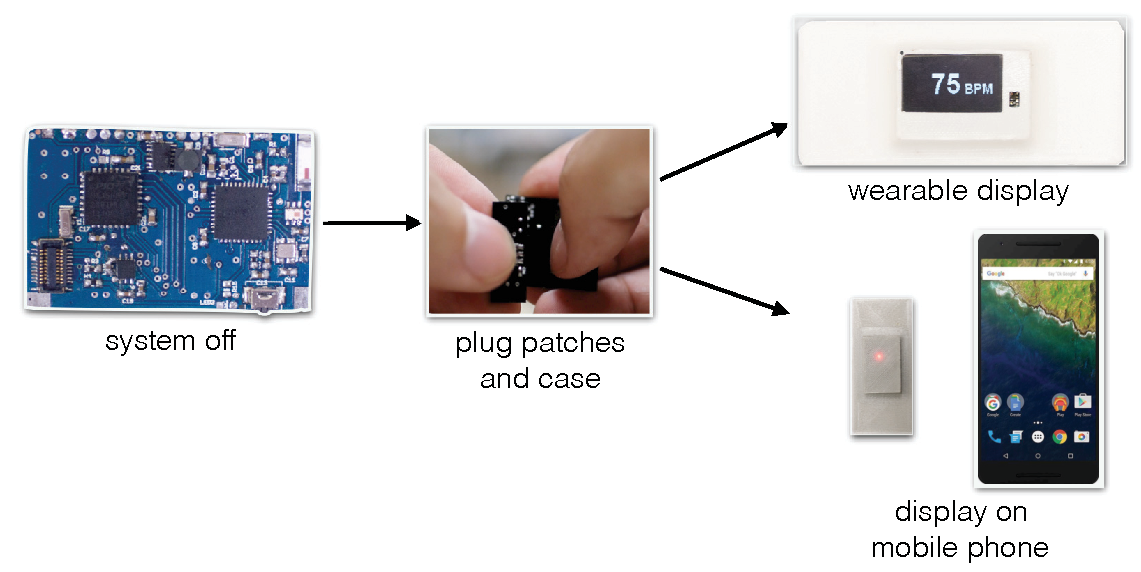
\includegraphics[width=14cm]{image/fig_config.ps}
\caption{The steps of configuration for data visualization. (a) System off. (b) Assembly: stacking patches and casing. (c) display on interaction patch. (d) display on mobile phone.}
\label{fig_config}
\end{figure}

\subsection{Configuration}
BioScope platform allows users to easily configure the system for collecting sensory data and receiving feedback from chosen patches with simple steps. We provide a mobile app running on top of Android for data configuration and data visualization. 
The main steps of configuration for data visualization is shown in Figure \ref{fig_config}. 

\subsubsection{System off} 
This is the initial state of the system, when the device is not applied a power source, i.e., install/recharge battery, or user configures the device to turn off the device.
As well as many off-the-shelf electronic products, the device doesn't have an on/off switch to shutdown the device. 
Instead, the system will enter to low power mode, because the consumed current in low power mode is negligible ($\sim$16 uA). 
The device will be turned to system off mode caused by two conditions: (1) pressing reset button on the device then idle for one minute, and (2) receiving the off command from mobile phone.
In low power mode, the microcontroller switches to secondary oscillator with low system frequency (32.768kHz) and turns off all internal components of the microcontroller for power saving. The device can only be waked up by external interrupt in system off mode.

\subsubsection{Assembly: Stack patches and casing} 
User can choose needed sensor patches and components to construct a customized device by simply stacking patches on the mainboard. Then the device is placed into a 3D printing case with the elastic filaments, e.g., bandage case.
When the device is booted, the system will blink the on-board LED and scan stacked patches on the mainboard through I2C and SPI bus. For the patches with I2C bus, the system will query the specific addresses defined in the BioScope system to check whether the patch is attached. For the patches with SPI bus, the system will query the connected patch by setting each slave select pin to high voltage individually. Thus, the system can automatically determine attached patches without users' effort to manually input the chosen patches.

\subsubsection{Display data}
The mobile phone is used as a terminal for configuring device and visualizing sensory data via Bluetooth radio.
The mobile phone is the central and the BioScope device is peripheral in the wireless topology.
After stacking the chosen patches and casing, user can use the mobile phone to establish the connection with device.
Then user can configure the mobile phone to display sensory data on the screen.

The device can also operate without communication with the mobile phone.
When the interaction patch is detected on the I2C bus, the system will run the corresponding process for basic sensing and feedback functions with wearable display.
Users can switch and control the displayed sensory data through the touchless gesture sensor on the interaction patch.
The system also allows the device to be further configured and accessed through the user interface on mobile phone as well.

\subsection{User Interface on Mobile Device}
The mobile device is versatile and pervasive in our daily life.
Therefore, we built a mobile app running on top of Android platform to facilitate data visualization and device configuration.
\vspace{10pt}
\newline
\textit{Device scan:}
\newline
The first page (Figure ? (?)) of the mobile app shows the BioScope devices nearby. The device without specific prefix in device ID is filtered out. 
\vspace{10pt}
\newline
\textit{Attached patches:}
\newline
When user selects a device ID, the mobile device attempts to connect with device. 
The mobile app will list all attached patches on the screen when the connection is established Figure ?(?).
\vspace{10pt}
\newline
\textit{Select function:}
\newline
A patch may have multiple functions, user can configure and visualize the data of each function separately (Figure ?(?)).
If the check button of each function in the list is checked, the sensory data will be logged in the storage of mobile device.
User can export these log data to PC for further analysis.
\vspace{10pt}
\newline
\textit{Config visualization:}
\newline
By choosing a function in the list, the data is visualized on the screen of the mobile phone. User can further config the data and data representations (Figure ?(?)).
\vspace{10pt}
\newline
\textit{Data Processing:}
\newline
Considering application need, wireless bandwidth and power efficiency, the sensory data should be processed in different ways.


%\subsection{Data Representation}

\section{Platform APIs}



\let\cleardoublepage\clearpage